\chapter{Code Breaking Games}
\label{ch:games}
We introduce a few examples of Code Breaking Games in this Chapter.
The counterfeit coin problem and Mastermind game are quite well known,
  the other examples are based on various board games or less known
  logic puzzles.
We briefly summarize related research for each game, give a list of
  references and discuss its application.

Our goal in this work is neither to answer the research questions nor
  to study possible generalizations.
Out goal is to create a general formalism and a computer language which could
  be used to describe arbitraty Code Breaking Game, if possible.
% This is a basic overview and what we had in mind when we designed the
% framework and language. It should be possible to formulate
% all the problems stated or
% We would love to create a tool that would be able to ...

%%%%%%%%%%%%%%%%%%%%%%%%%%%%%%%%%%%%%%%%%%%%%%%%%%%%%%%%%%%%%%%%%%%%%%%%%%%%%%%%
\section{The Counterfeit Coin}

\begin{wrapfigure}{r}{0.26\textwidth}
  \begin{center}
  \vspace{-5mm}
  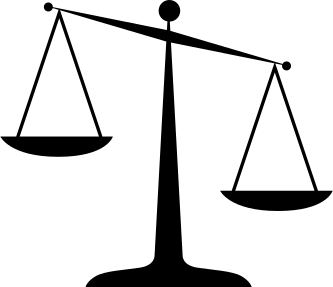
\includegraphics[width=0.23\textwidth]{pictures/scales.pdf}
  \vspace{-5mm}
  \end{center}
  \caption{Balance scales (illustrative image)\protect\footnotemark.}
  \vspace{-10mm}
\end{wrapfigure}
\footnotetext{Adapted from
  \texttt{http://pixabay.com/en/justice-silhouette-scales-law-147214},
  under CC0 1.0 Licence.}

The problem of finding a counterfeit coin among regular coins in the fewest
  number of weighings on a pair of scales balance is the folklore of
  recreational mathematics.

In all problems of this kind, you can use the scales only to weight the coins.
You put some coins on the left pan, the same number of coins on the right pan
  and get one of the 3 possible outcomes.
Either both the sides weight the same (denoted ``='')
  or the left side is lighter (``<''),
  or the right side is lighter (``>'').

The standard, easiest variant can be formulated as follows.

\begin{problem}[The nine coin problem] \label{pr:coins9}
You are given $n >= 3$ (typically 9) coins, all expect one have the same weight.
The counterfeit coin is known to be lighter.
Determine the coin in the minimal number of weightings.
\end{problem}

This problem is very easy as one can use \emph{ternary search} algorithm.
In short, we divide the coins into thirds, put one third agains another
  on scales.
If both sides weight the same, the counterfeit coin must be in the last third,
  otherwise it must be in the lighter third.
In this way, the size of search space reduces by a factor of 3 in one weighting,
  which is clearly optimal.

In 1940s, a more complicated variant was introduced by Grossman\cite{coins-grossman1945}.

%whether the counterfeit coin is underweight or overweight
\begin{problem}[The Twelve Coin Problem] \label{pr:coins12}
You are given $n >= 3$ (typically 12) coins, exactly one of which is counterfeit,
  but it is not known if it is heavier or ligher.
Determine the unique coin and its weight relavite to others
  in the minimal number of weightings.
\end{problem}

\begin{figure}
\includegraphics[width=\textwidth]{pictures/coins12.pdf}
\caption{Decision tree for The Twelve Coin Problem. \\
Leaf $x$ means that the coin number $x$ is lighter, $\underline{x}$ means that
the coin number $x$ is heavier.}
\label{fig:coins12tree}
\end{figure}

The optimal solution for $n=12$ requires 3 weightings and one of the optimal
  strategies is shown in \autoref{fig:coins12tree} as a decision tree.

The research usually focuses on bounds on the maximal value of $n$
  for which the problem can be solved in $w$ weighings, for a given $w$.
Thus a solution of a problem is usually formulated as a theorem like the
  following one.

\begin{theorem}[Dyson, \cite{coins-dyson1946}]\label{th:coins12}
There exists a scheme that determines the counterfeit coin and
  its type in \autoref{pr:coins12} with $w$ weighings,
  if and only if
  \[ 3 <= n <=\frac{3^w - 3}{2}. \]
\end{theorem}

\begin{proof}
We show the main part of the original Dyson's proof\cite{coins-dyson1946}
  here because of its elegant combinatorial idea.
We show a scheme for $n = \frac{1}{2}(3^w - 3)$.

Let us number the coins from $1$ to $n$.
To a coin number $i$, we assing
  two labels from $\{0,1,2\}^w$ -- those corresponding the numbers
  $i$ and $3^w - 1 - i$ in ternary form.
Notice that all possible labels are used exactly once, except for $0^w, 1^w$
  and $2^w$, which were not assigned to any coin.
The labeling has the property that you can
  get one label of a coin from the other by substituing $0$ by $2$ and $2$ by $0$.

A label is called ``clockwise'' if the first change of digit in it is
the change from $0$ to $1$, from $1$ to $2$, or from $2$ to $0$.
Otherwise, it is called ``anticlockwise''.
Thanks to the property we mentioned, one of the labels of a coin is always
  clockwise and the other is anticlockwise.

Let $C(i, d)$ be a set of coins such that $i$-th symbol in
  its clockwise label is $d$.
Since a permutation changing $0$ to $1$, $1$ to $2$ and $2$ to $0$ transfers
  coins from $C(i,0)$ to $C(i,1)$,
        from $C(i,1)$ to $C(i,2)$ and
        from $C(i,2)$ to $C(i,0)$,
  all the sets $C(i, d)$ contain exactly $n/3$ coins.
Now, let $i$-th experiment be the weighing of the coins $C(i,0)$ agains $C(i, 2)$.
It remains to show that the experiments uniquely determine the counterfeit coin.
Let $a_i$ be 0, 1, or 2 if the result of $i$-th experiment is
  left side is lighter, both are the same, or right side is lighter, respectively.

If the counterfeit code is overweight, the $i$-th symbol of its clockwise label
  must be $a_i$. On the other hand, if it is underweight, the $i$-th symbol of
  its anticlockwise label must be $a_i$.
The solution of the problem is therefore the coin with the label $a_1a_2...a_w$
  and is heavier than others if and only if this label is clockwise.
\autoref{fig:coins12scheme} shows an example of the construction for $n = 12 = \frac{1}{2}(3^3 - 3)$.

The case $n < \frac{1}{2}(3^w - 3)$ can be done similarly with some modifications
  to the labelling.
However, the scheme makes use of a genuine coin that was discovered in the first
  weighing and, therefore the following experiments depend on the outcome of
  the first.
Finally, the prove that the coin cannot be detected if
  $n > \frac{1}{2}(3^w - 3)$ can be done using information theory.

\begin{figure}
\begin{center}
\includegraphics{pictures/coins12-th.pdf}
\end{center}
\caption{Demonstration of the ternary label construction for $n=12$.}
\label{fig:coins12scheme}
\end{figure}
\end{proof}

Naturally, the problem was generalized in various ways and
  studied by many authors.
In ``Coin-Weighing Problems''\cite{coins-cwproblems1995}, Guy and Nowakovski
  gave a great overview of the research in the area until 1990s
  with an extensive list of references.
We list the most interesting variants and generalizations below.

\begin{itemize}
\item \textbf{Weight of counterfeit coin.}
  Either it is known whether the counterfeit coin is lighter or heavier,
  or it is not.
  The first one allows for more generalizations due to its simpler nature
  but both problems have been heavily researched.
\item \textbf{Number of counterfeit coins.}
  In the most common case, there is exactly one counterfeit coin,
    which allows for natural generalizations.
  First, a variant of \autoref{pr:coins9} with 2 or 3 counterfeit coins
   was studied\cite{coins-2fakes}\cite{coins-3fakes},
  then with $m$ counterfeit coins in general\cite{coins-mfakes}.
  Some authors studied the problem for unknown number of counterfeit coins
  \cite{coins-unknownfakes},
  or for \emph{at most} $m$ counterfeit coins\cite{coins-atmostfakes}.
\item \textbf{Additional regular coin(s).}
  In some cases, it may help if you are given an additional coin (or more coins),
    which is guaranteed not to be counterfeit.
  For example, for $n = 13$ in \autoref{pr:coins12}, you need 4 weightings.
  However, if you are given this one extra coin, you can determine the
    solve in just 3 weightings\cite{coins-dyson1946}.
\item \textbf{Non-adaptive strategies.}
  In this popular variant of the problem you have to announce all experiments
    in advance and then just collect the result.
  In other words, later weighings must not depend on the outcomes of the earlier weighings.
  Notice that the scheme constructed in the proof of \autoref{th:coins12} for
  $n = \frac{1}{2}(3^w - w)$ is indeed non-adaptive.
  However, the original proof uses an adaptive scheme for a smaller $n$.
  This was later fixed, showing that there always exists an optimal scheme for
  \autoref{pr:coins12} which is non-adaptive\cite{coins-nonadaptive}.
\item \textbf{Unreliable balance.}
  This generalization introduces the possibility that
  one (or more) answers may be erroneous.
  The problem of errors/lies in general search problems is well studied,
    see \cite{games-lies}.
  It was applied on the counterfeit coin problem (\autoref{pr:coins9} variant)
  in \cite{coins-unreliable} with at most one erroneous outcome or in
  \cite{coins-unreliable} with two.
\item \textbf{Multi-arm balance.}
  In this variant, your balance has $k$ arms. You put the same number of coins
  on every arm and you get either the information that all
  weight the same or which arm is lighter or heavier
  than others\cite{coins-multiplearm}.
\item \textbf{Parallel weighting.}
  In this generalization, you have 2 (or $k$, in general)
    balance scales, you can weight different coins on
    the two scales simultaneously and it counts
    as only one experiment\cite{coins-parallel}.
  The motivation here is that the weighing takes some not insignificant time,
  you have more scales and strive to minimize the time the whole process takes.
\end{itemize}

%%%%%%%%%%%%%%%%%%%%%%%%%%%%%%%%%%%%%%%%%%%%%%%%%%%%%%%%%%%%%%%%%%%%%%%%%%%%%%%%
\section{Mastermind}

\emph{Mastermind} is a classical code-breaking board game for 2 players,
  invented by Mordecai Meirowitz in 1970.
One player has the role of a \emph{codemaker} and the other of a \emph{codebreaker}.
First, the codemaker chooses a secret code of $n$ pegs of $c$ colors.
Then a codebreaker tries to reveal the code by making guesses.
The codebreaker evaluates the guesses using black and white markers.
Black markers correspond to positions at which the code and the guess matches,
  white marker correspond to a color peg which is both in the code and the guess,
  but at different positions.
The markers in the answer are not ordered, so the codebreaker does not know,
  which marker correspond to which peg in the guess.
The codebreaker strives to minimize the number of guesses.

\begin{wrapfigure}{r}{0.32\textwidth}
  \vspace{-10mm}
  \begin{center}
  \includegraphics[width=0.25\textwidth]{pictures/mastermind.png}
  \vspace{-5mm}
  \end{center}
  \caption{Mastermind game (illustrative image)\protect\footnotemark.}
  \vspace{15mm}
\end{wrapfigure}
\footnotetext{Adapted from \texttt{http://commons.wikimedia.org/wiki/File:Mastermind\_beispiel.svg}, by Thomas Steiner under GFDL.}

More formally, let $C$ be a set of colors of size $c$.
Define a distance $d : C^n\times C^n -> \Nseto\times\Nseto$
  of two color sequences by $d(u, v) = (b, w)$, where
\[
b = |\{ i \in\Nset \| u[i] = v[i] \}|
\]
\[
w = \sum_{j\in C} \min\big(\big|\{ i \| u[i] = j \}\big|,\;
                           \big|\{ i \| v[i] = j\}\big|\big)  - b.
\]
If the codemaker's secret code is $h$ and the codebreaker's guess is $g$,
  the guess should be evaluated with $b$ black pegs and $w$ white pegs, where
  $(b,w) = d(h,g)$.
Therefore, if the codebreaker have guessed $g_1, g_2, ..., g_k$ and the results
  were $(b_1,w_1), ..., (b_k, w_k)$,
  the search space is reduced to codes
  \[
  \{ u\in C^n \| \forall i<=k.\; d(u, g_i) = (b_i,w_i)\}.
  \]

Another way of looking at the guess evaluation is using
  \emph{maximal matching} of the pegs in the code $h$ and the guess $g$.
A matching is a set of pair-wise non-adjacent edges between
  pegs in the code (represented by $(0,i)$ for $1<=i<=n$) and
  pegs in the guess (represented by $(1,i)$ for $1<=i<=n$).
Let $M$ be a maximal matching such that
\begin{enumerate}
\item an edge connects only pegs of the same color, i.e. if $((0,i),(1,i))\in M$, then $h[i] = g[j]$, and
\item if $h[i] = g[i]$ then $((0,i),(1,i))\in M$.
\end{enumerate}
Maximal means that no edge can be added without breaking one of the conditions.
The edges in $M$ correspond to the markers in the response,
  a marker being black if and only if the corresponding edge connects $(0,i)$
  with $(1,i)$ for some $i$.

\subsection{Variants and generalizations}

The old game of \emph{Bulls and Cows} has very similar principle to Mastermind,
  it only uses letters instead of colors and does not allow repetitions.

Static Mastermind is a variant of the game in which all guesses
  must be made at one go.
The codebreaker prepares a set of guesses,
  then the codemakers evaluates each one as usual and
  the codebreaker must determine the code from the outcomes.
This corresponds to so-called \emph{non-adaptive} strategies
  for The Counterfeit Coin Problem.

\subsection{Known results and related research}

\emph{one-step look-ahead} heuristics, tabulka...


%%%%%%%%%%%%%%%%%%%%%%%%%%%%%%%%%%%%%%%%%%%%%%%%%%%%%%%%%%%%%%%%%%%%%%%%%%%%%%%%
\section{Other Problems and Applications}
\subsection{Black Box}
% obrazky
\subsection{Bags of Gold}
% obrazky

\subsection{Code 777}
% obrazky - kartičky set

\subsection{String matching}
% aplikace geno fenotyp

\subsection{Generalized Mastermind}
% aplikace - pin cracking


